\documentclass[12pt,fleqn]{book}

\usepackage{titlesec}
\usepackage{caption}
\usepackage{multirow}

\titleformat{\chapter}[display]
  {\normalfont\huge\bfseries}{}{0pt}{\Huge}
\titlespacing{\chapter}
  {0pt}{10pt}{40pt}

	\newenvironment{amatrix}[1]{%
	  \left[\begin{array}{@{}*{#1}{r}|r@{}}
	}{%
	  \end{array}\right]
	}

%%%%% INKSCAPE BEGIN

\usepackage{import, xifthen, pdfpages, transparent}
\newcommand{\incfig}[2][1]{%
    \def\svgwidth{#1\columnwidth}
    \import{./figures/}{#2.pdf_tex}
}
\pdfsuppresswarningpagegroup=1
%%%%% INKSCAPE END


\usepackage{amsmath,amssymb,amsfonts,graphicx,tasks,tikz,pgfplots}
\usetikzlibrary{arrows,angles,quotes}
\pgfplotsset{compat=1.17}

\usepackage[a4paper,margin=0.5in,footskip=.5cm]{geometry}

\setlength\parindent{0pt}

\usepackage{amsmath,amssymb,amsfonts,graphicx,tasks,tikz,pgfplots}
\usetikzlibrary{arrows,quotes}

\usepackage{array}
\newcommand{\PreserveBackslash}[1]{\let\temp=\\#1\let\\=\temp}
\newcolumntype{C}[1]{>{\PreserveBackslash\centering}p{#1}}
\newcolumntype{R}[1]{>{\PreserveBackslash\raggedleft}p{#1}}
\newcolumntype{L}[1]{>{\PreserveBackslash\raggedright}p{#1}}

\newcommand{\graph}[8]{
\begin{tikzpicture}[baseline=(current bounding box.north)]
  \begin{axis}[
    axis lines=middle,
    axis line style={very thick},
    grid style={thin,densely dotted,black!50},
    grid=major,
      xtick distance=#6, ytick distance=#6,
      xmin=#2-.2, xmax=#3+.2,
      ymin=#4-.2, ymax=#5+.2,
      xlabel=$x$,
      ylabel=$y$,
      #7]
      \addplot[
      domain=#2:#3,
      samples=500,#8]
      (x,{#1});
    \end{axis}
  \end{tikzpicture}
}

\newcommand{\graphtwo}[9]{
\begin{tikzpicture}[baseline=(current bounding box.north)]
  \begin{axis}[
    axis lines=middle,
    axis line style={very thick},
    grid style={thin,densely dotted,black!50},
    grid=major,
      xtick distance=#7, ytick distance=#7,
      xmin=#3-.2, xmax=#4+.2,
      ymin=#5-.2, ymax=#6+.2,
      xlabel=$x$,
      ylabel=$y$,
      #8]
      \addplot[
      domain=#3:#4,
      samples=500,#9]
      (x,{#1});
      \addplot[
      domain=#3:#4,
      samples=500,#9]
      (x,{#2});
    \end{axis}
  \end{tikzpicture}
}

\newcommand{\curve}[7]{% function, xmin, xmax, ymin, ymax, 
\begin{tikzpicture}[baseline=(current bounding box.north)]
  \begin{axis}[
    axis lines=middle,
    axis line style={very thick},
    grid style={thin,densely dotted,black!50},
    grid=major,
    xticklabels={},
	yticklabels={},
	xtick distance=1, ytick distance=1,
	extra x ticks={#3},
	extra y ticks={#5},
      xmin=#2-.2, xmax=#3+.2,
      ymin=#4-.2, ymax=#5+.2,
      xlabel=$x$,
      ylabel=$y$,
      #6]
      \addplot[
      domain=#2:#3,
      samples=500,#7]
      (x,{#1});
    \end{axis}
  \end{tikzpicture}
}

\newcommand{\blankgraph}[6]{
\begin{tikzpicture}[baseline=(current bounding box.north)]
  \begin{axis}[
    width=#5in,height=#6in,
    axis lines=middle,
    axis line style={very thick},
    grid style={thin,densely dotted,black!50},
    grid=major,
    xticklabels={},
	yticklabels={},
	xtick distance=1, ytick distance=1,
	extra x ticks={#2},
	extra y ticks={#4},
      xtick distance=1, ytick distance=1,
      xticklabels={1},
      yticklabels={1},
      xmin=#1-.2, xmax=#2+.2,
      ymin=#3-.2, ymax=#4+.2,
      xlabel=$x$,
      ylabel=$y$]
    \end{axis}
  \end{tikzpicture}
}

\newcommand{\blankaxes}[2]{
\begin{tikzpicture}[baseline=(current bounding box.north)]
  \begin{axis}[
    width=#1in,height=#2in,
    axis lines=middle,
    axis line style={very thick},
    grid=major,
    xtick distance=2, ytick distance=2,
    xmin=-1, xmax=1,
    ymin=-1, ymax=1,
    xlabel=$x$,
    ylabel=$y$]
  \end{axis}
\end{tikzpicture}
}

\newcommand{\ds}{\displaystyle}

\newcommand{\lr}[1]{\left(#1\right)}

% \usepackage{amsthm}
% \theoremstyle{definition}
% \newtheorem{problem}{}
% \counterwithin*{problem}{section}
% \renewcommand{\theproblem}{\thesubsection.\arabic{problem}}
%
% \newtheorem*{solutionx}{\thesolutionnumber}
% \ExplSyntaxOn
% \tl_new:N \g_gargantuar_solution_tl
%
% \NewDocumentEnvironment{solution}{+b}
%  {
%   \tl_gput_right:Nx \g_gargantuar_solution_tl
%    {
%     \printsolution{\theproblem}{ \exp_not:n { #1 } }
%    }
%  }
%  {}
% \NewDocumentCommand{\printsolutions}{}
%  {
%   \tl_use:N \g_gargantuar_solution_tl
%   \tl_gclear:N \g_gargantuar_solution_tl
%  }
% \NewDocumentCommand{\printsolution}{m +m}
%  {
%   \cs_set:Npn \thesolutionnumber { #1 }
%   \begin{solutionx} #2 \end{solutionx}
%  }
% \ExplSyntaxOff
% \makeatother
%
% \newcommand{\prb}[1]{\begin{problem}#1\end{problem}}
% \newcommand{\sol}[1]{\begin{solution}#1\end{solution}}


\newcommand{\stdangle}[1]{
	\begin{tikzpicture}
		\draw[very thick,->] (-2,0)coordinate(B)--(2,0)coordinate(C);
		\draw[very thick,->] (0,-2)--(0,2);
		\draw [->] (0,0)coordinate(O)->(#1:2)coordinate(A);
		\pic [draw, angle radius=8mm, angle eccentricity=2] {angle=C--O--A};
	\end{tikzpicture}
	}

\pagestyle{plain}
\usepackage[lastexercise,answerdelayed]{exercise}
\usepackage{totcount}
\regtotcounter{Exercise} % register the counter for getting the total
\usepackage{chngcntr}
\counterwithin{Exercise}{chapter}
\counterwithin{Answer}{chapter}
\usepackage{xassoccnt}
\NewTotalDocumentCounter{totalex}
\usepackage{titleref}
\usepackage{etoolbox}

\renewcommand{\ExerciseHeader}{ \stepcounter{totalex}\ifnumcomp{\value{Exercise}}{=}{1}{\ifnumcomp{\thechapter}{=}{1}{}{\vspace{10pt}}\noindent\Large\textbf{Exercises}\par\vspace{10pt}}{}\noindent\normalsize\bfseries\ExerciseHeaderNB\ExerciseHeaderDifficulty.}
\renewcommand{\AnswerHeader}{\ifnumcomp{\value{Exercise}}{=}{1}{\ifnumcomp{\thechapter}{=}{1}{}{\vspace{10pt}}\noindent\Large\textbf{Section\ \thechapter\ Solutions}\par\vspace{10pt}}{}\noindent\normalsize\bfseries\ExerciseHeaderNB.\ }

\usepackage{hyperref}

\newcommand{\prb}[1]{\begin{Exercise}\parbox[t]{\textwidth-5em}{#1}\end{Exercise}}
\newcommand{\sol}[1]{\begin{Answer}\parbox[t]{\textwidth-5em}{#1}\end{Answer}}


% generated by the Super Figure vscode extension. May we stand on the shoulder's of giants
\usepackage{import}
\newcommand{\incsvg}[2]{%
	\def\svgwidth{\columnwidth}
	\graphicspath{{#1}}
	\input{#2.pdf_tex}
}

\begin{document}
\noindent
\thispagestyle{empty}
Grade 10 Advanced Math \hfill Name: \hspace{2in}
\medskip\hrule
\noindent

\vfill

\begin{center}
	{\bf \huge Chapter 4: Trigonometric Functions}
\end{center}

\vfill
\vfill

\clearpage

\setcounter{page}{1}

\chapter*{Introduction}
The past three chapters were about functions that grow and grow and grow.  Some of the functions we saw grew at a constant rate, some functions grew in a way that their slope increased at a constant rate, and some functions grew in a way that their slope changed at the same rate that the function itself was growing.  Which one was which?
\\[1em]
Trigonometric functions are completely different than that.  Trigonometric functions \emph{oscilate}.
\\[1em]
In the final chapter of our course, we will discuss the three primary trigonometric functions, how they are defined, how we can use them to solve problems about triangles, and how they relate to circles.\\
We will end the chapter and this course learning about other geometric figures and how to caluclate their surface area and volume.
\\
\chapter{Angles}
An angle in standard position:
\\[5em]
Initial and terminal arms:
\\[5em]
Reference angle:
\\[5em]
Coterminal angles:
\\[5em]
Quadrants:
\clearpage
\section*{Examples}
\clearpage
\clearpage
\prb{ Sketch each angle in standard position.
	\begin{tasks}(3)
		\task $100^\circ$ 	\\ \blankaxes{2}{2}
		\task $80^\circ$ 	\\ \blankaxes{2}{2}
		\task $200^\circ$ 	\\ \blankaxes{2}{2}
		\task $320^\circ$ 	\\ \blankaxes{2}{2}
		\task $270^\circ$ 	\\ \blankaxes{2}{2}
		\task $450^\circ$ 	\\ \blankaxes{2}{2}
		\task $-45^\circ$ 	\\ \blankaxes{2}{2}
		\task $-730^\circ$ 	\\ \blankaxes{2}{2}
		\task $3645^\circ$  \\ \blankaxes{2}{2}
	\end{tasks}
}
\sol{
	\begin{tasks}(3)
		\task \\ \stdangle{100}
		\task \\ \stdangle{80}
		\task \\ \stdangle{200}
		\task \\ \stdangle{320}
		\task \\ \stdangle{270}
		\task \\ \incfig[0.8]{std450}
		\task \\
		\begin{tikzpicture}
			\draw[very thick,->] (-2,0)coordinate(B)--(2,0)coordinate(C);
			\draw[very thick,->] (0,-2)--(0,2);
			\draw [->] (0,0)coordinate(O)->(-45:2)coordinate(A);
			\pic [draw, angle radius=8mm, angle eccentricity=2] {angle=A--O--C};
		\end{tikzpicture}
		\task \\ \incfig[0.8]{std-730}
		\task \\ \incfig[0.8]{std3645}
	\end{tasks}
}
\prb{
	In which quadrant does the terminal arm of each angle in standard position lie?
	\begin{tasks}(3)
		\task $48^{\circ}$
		\task $300^{\circ}$
		\task $185^{\circ}$
		\task $75^{\circ}$
		\task $220^{\circ}$
		\task $160^{\circ}$
	\end{tasks}
}
\sol{
	\begin{tasks}(3)
		\task $48^{\circ}$ is is quadrant I.
		\task $300^{\circ}$ is in quadrant IV.
		\task $185^{\circ}$ is in quadrant III.
		\task $75^{\circ}$ is in quadrant I.
		\task $220^{\circ}$ is in quadrant III.
		\task $160^{\circ}$ is in quadrant II.
	\end{tasks}
}

\prb{Find the reference angle.
	\begin{tasks}(5)
		\task $32^{\circ}$ 		\vspace{1in}
		\task $-32^{\circ}$ 	\vspace{1in}
		\task $113^{\circ}$ 	\vspace{1in}
		\task $-113^{\circ}$ 	\vspace{1in}
		\task $218^{\circ}$ 	\vspace{1in}
		\task $-218^{\circ}$ 	\vspace{1in}
		\task $304^{\circ}$ 	\vspace{1in}
		\task $-304^{\circ}$ 	\vspace{1in}
		\task $832^{\circ}$ 	\vspace{1in}
		\task $-1213^{\circ}$ 	\vspace{1in}
	\end{tasks}
}
\sol{
	\begin{tasks}(5)
		\task $32^{\circ}$
		\task $32^{\circ}$
		\task $67^{\circ}$
		\task $67^{\circ}$
		\task $38^{\circ}$
		\task $38^{\circ}$
		\task $56^{\circ}$
		\task $56^{\circ}$
		\task $68^{\circ}$
		\task $47^{\circ}$
	\end{tasks}
}
\prb{
Determine the measure of the three other angles in standard position, $0^{\circ}<\theta<360^{\circ}$, that have a reference angle of
\begin{tasks}(2)
	\task $45^{\circ}$
	\task $60^{\circ}$
	\task $30^{\circ}$
	\task $75^{\circ}$
\end{tasks}
}
\sol{
\begin{tasks}(2)
	\task $135^{\circ}, 225^{\circ}$, and $315^{\circ}$.
	\task $120^{\circ}, 240^{\circ}$, and $300^{\circ}$.
	\task $150^{\circ}, 210^{\circ}$, and $330^{\circ}$.
	\task $105^{\circ}, 255^{\circ}$, and $285^{\circ}$.
\end{tasks}
}
\prb{
	If quadrants II and III have the same reference angles and one of the standard position angles is $214^{\circ}$, what is the other smallest positive standard position angle?
	\vspace{3em}}
\sol{$146^\circ$}
\prb{
	A windshield wiper has a length of $50 \mathrm{~cm}$. The wiper rotates from its resting position at $30^{\circ}$, in standard position, to $150^{\circ}$. Determine the exact horizontal distance that the tip of the wiper travels in one swipe.
	\vspace{15em}
	}
\sol{
	Consider the following diagram.\\
	\incfig[0.4]{wiper-blade}
	\begin{align*}
		\cos 30^{\circ}    & =\frac{x}{50} \\
		\frac{\sqrt{3}}{2} & =\frac{x}{50} \\
		x                  & =25 \sqrt{3}
	\end{align*}
	By symmetry, the horizontal distance that the tip of the wiper travels in one swipe will be $2 x$, or $50 \sqrt{3} \mathrm{~cm}$.
}
\prb{
	Paul and Gail decide to use a Cartesian plane to design a landscape plan for their yard. Each grid mark represents a distance of $10 \mathrm{~m}$. Their home is centred at the origin. There is a red maple tree at the point $(3.5,2)$. They will plant a flowering dogwood at a point that is a reflection in the $y$-axis of the position of the red maple. A white pine will be planted so that it is a reflection in the $x$-axis of the position of the red maple. A river birch will be planted so that it is a reflection in both the $x$-axis and the $y$-axis of the position of the red maple.\\
	\[
		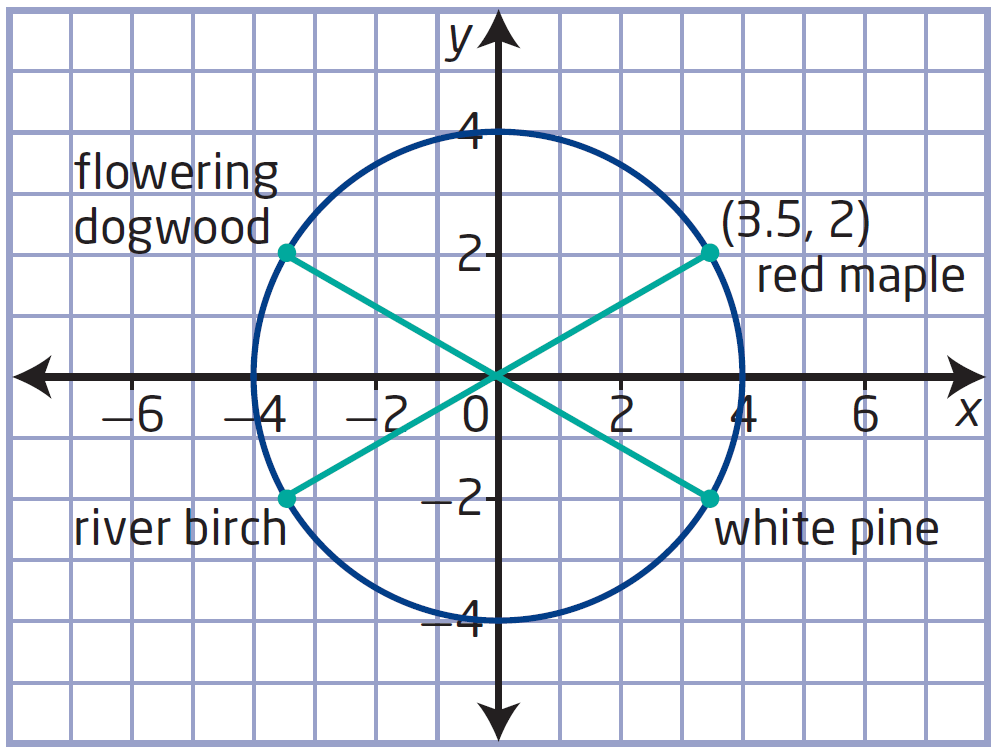
\includegraphics[width=3in]{figures/trees.png}
	\]
	\begin{tasks}(1)
		\task Determine the coordinates of the trees that Paul and Gail wish to plant.
		\vspace{10em}
		\task Determine the angles in standard position if the lines drawn from the house to each of the trees are terminal arms. Express your answers to the nearest degree.
		\vspace{10em}
		\task What is the actual distance between the red maple and the white pine?
		\vspace{10em}
	\end{tasks}
}
\sol{
	\begin{tasks}(1)
		\task The coordinates of the other three trees are found using symmetries of the diagram: flowering dogwood $(-3.5,2)$, river birch $(-3.5,-2)$, white pine $(3.5,-2)$.
		\task For the red maple,
		\begin{align*}
			\tan \theta & =\frac{2}{3.5}                        \\
			\theta      & =\tan ^{-1}\left(\frac{2}{3.5}\right) \\
			\theta      & =29.744 \ldots
		\end{align*}
		The angle in standard position for the red maple is $30^{\circ}$, to the nearest degree.
		Then, the angle in standard position for the flowering dogwood is $180^{\circ}-30^{\circ}$ or $150^{\circ}$, to the nearest degree. The angle in standard position for the river birch is $180^{\circ}+30^{\circ}$ or $210^{\circ}$, to the nearest degree. The angle in standard position for the white pine is $360^{\circ}-$ $30^{\circ}$ or $330^{\circ}$, to the nearest degree.
		\task On the grid, there are 4 vertical units of distance between the red maple and the white pine. Since each grid mark represents $10 \mathrm{~m}$, the distance between these two trees is $40 \mathrm{~m}$.
	\end{tasks}
}
\chapter{Trigonometric Ratios}
If the point $(x,y)$ lies on the terminal arm of angle $\theta$, then $r=\sqrt{x^2+y^2}$, and:
\[
	\sin\theta = \hspace{1in} \cos\theta=\hspace{1in} \tan\theta =
\]
The CAST rule:
\[ 
	\blankaxes{2}{2}
\]
The following trigonometric ratios are worth memorizing:
\[
\begin{array}{rrrrrr}
	\sin 0^\circ =& \hspace{.5in} \sin 30^\circ =& \hspace{.5in} \sin 45^\circ =& \hspace{.5in} \sin 60^\circ =& \hspace{.5in} \sin 90^\circ =& \hspace{.5in}\\[3em]
	\cos 0^\circ =& \hspace{.5in} \cos 30^\circ =& \hspace{.5in} \cos 45^\circ =& \hspace{.5in} \cos 60^\circ =& \hspace{.5in} \cos 90^\circ =& \hspace{.5in}\\[3em]
	\tan 0^\circ =& \hspace{.5in} \tan 30^\circ =& \hspace{.5in} \tan 45^\circ =& \hspace{.5in} \sin 60^\circ =& \hspace{.5in} \tan 90^\circ =& \hspace{.5in}\\[3em]
\end{array}
\]
\clearpage
\section*{Examples}
\clearpage
\ 
\clearpage 
\prb{Below are angles in standard position with a point on each terminal arm.  Write the three primary trigonometric ratios (sine, cosine, and tangent) of each angle in standard position.  Hint: find $r$ using the Pythagorean Theorem, and state $x$ and $y$.
	\begin{tasks}(2)
		\task\\
		\incfig[0.8]{term43}
		\task\\
		\incfig[0.8]{term-25}
		\task\\
		\incfig{term-1-sqrt3}
		\task\\
		\incfig{term2-sqrt5}
		\task\\
		\incfig{term-30}
		\task\\
		\incfig{term0-2}
	\end{tasks}
}
\sol{
	\begin{tasks}(2)
		\task $\sin \theta=\frac{3}{5}, \cos \theta=\frac{4}{5}, \tan \theta=\frac{3}{4}$
		\task $\sin \theta=\frac{5}{\sqrt{29}}, \cos \theta=-\frac{2}{\sqrt{29}}, \tan \theta=-\frac{5}{2}$
		\task $\sin \theta=-\frac{\sqrt{3}}{2}, \cos \theta=-\frac{1}{2}, \tan \theta=\sqrt{3}$
		\task $\sin \theta=-\frac{\sqrt{5}}{3}, \cos \theta=\frac{2}{3}, \tan \theta=-\frac{\sqrt{5}}{2}$
		\task $\sin \theta=0, \cos \theta=-1, \tan \theta=0$
		\task $\sin \theta=-1, \cos \theta=0, \tan \theta$ is undefined
	\end{tasks}
}
\prb{
	If $\theta$ is in standard position and the given point is on the terminal side of $\theta$, find the values of $\sin \theta, \cos \theta$, and $\tan \theta$.
	\begin{tasks}(3)
		\task $(3,-4)$
		\vspace{8.5em}
		\task $(-12,5)$
		\vspace{8.5em}
		\task $(-7,-24)$
		\vspace{8.5em}
		\task $(8,15)$
		\vspace{8.5em}
		\task $(-2 \sqrt{3}, 2)$
		\vspace{8.5em}
		\task $(\sqrt{2}, \sqrt{7})$
		\vspace{8.5em}
		\task $(-3,-3)$
		\vspace{8.5em}
		\task $(0,4)$
		\vspace{8.5em}
		\task $(-2,0)$
		\vspace{8.5em}
		\task $(-\sqrt{5}, 2)$
		\vspace{8.5em}
		\task $(-5,5)$
		\vspace{8.5em}
		\task $(-2 \sqrt{2}, 1)$
		\vspace{8.5em}
		\task $(-40,-9)$
		\vspace{8.5em}
		\task $(9,-40)$
		\vspace{8.5em}
		\task $(2 \sqrt{2}, 8)$
		\vspace{8.5em}
		\task $(-3, \sqrt{3})$
		\vspace{8.5em}
		\task $(-\sqrt{11},-\sqrt{5})$
		\vspace{8.5em}
		\task $(\sqrt{17}, 2 \sqrt{2})$
		\vspace{8.5em}
	\end{tasks}
}
\sol{
	\begin{tasks}(2)
		\task $\sin \theta=-\frac{4}{5}, \cos \theta=\frac{3}{5}, \tan \theta=-\frac{4}{3}$
		\task $\sin \theta=\frac{5}{13}, \cos \theta=-\frac{12}{13}, \tan \theta=-\frac{5}{12}$
		\task $\sin \theta=-\frac{24}{25}, \cos \theta=-\frac{7}{25}, \tan \theta=\frac{24}{7}$
		\task $\sin \theta=\frac{15}{17}, \cos \theta=\frac{8}{17}, \tan \theta=\frac{15}{8}$
		\task $\sin \theta=\frac{1}{2}, \cos \theta=-\frac{\sqrt{3}}{2}, \tan \theta=-\frac{1}{\sqrt{3}}$
		\task $\sin \theta=\frac{\sqrt{7}}{3}, \cos \theta=\frac{\sqrt{2}}{3}, \tan \theta=\frac{\sqrt{7}}{\sqrt{2}}$
		\task $\sin \theta=-\frac{1}{\sqrt{2}}, \cos \theta=-\frac{1}{\sqrt{2}}, \tan \theta=1$
		\task $\sin \theta=1, \cos \theta=0, \tan \theta$ is undefined
		\task $\sin \theta=0, \cos \theta=-1, \tan \theta=0 \quad$
		\task $\sin \theta=\frac{2}{3}, \cos \theta=-\frac{\sqrt{5}}{3}, \tan \theta=-\frac{2}{\sqrt{5}}$
		\task $\sin \theta=\frac{1}{\sqrt{2}}, \cos \theta=-\frac{1}{\sqrt{2}}, \tan \theta=-1$
		\task $\sin \theta=\frac{1}{3}, \cos \theta=-\frac{2 \sqrt{2}}{3}, \tan \theta=-\frac{1}{2 \sqrt{2}}$
		\task $\sin \theta=-\frac{9}{41}, \cos \theta=-\frac{40}{41}, \tan \theta=\frac{9}{40}$
		\task $\sin \theta=-\frac{40}{41}, \cos \theta=\frac{9}{41}, \tan \theta=-\frac{40}{9}$
		\task $\sin \theta=\frac{2 \sqrt{2}}{3}, \cos \theta=\frac{1}{3}, \tan \theta=2 \sqrt{2}$
		\task $\sin \theta=\frac{1}{2}, \cos \theta=-\frac{\sqrt{3}}{2}, \tan \theta=\frac{-\sqrt{3}}{3}$
		\task $\sin \theta=-\frac{\sqrt{5}}{4}, \cos \theta=-\frac{\sqrt{11}}{4}, \tan \theta=\frac{\sqrt{55}}{11}$
		\task $\sin \theta=\frac{2 \sqrt{2}}{5}, \cos \theta=\frac{\sqrt{17}}{5}, \tan \theta=\frac{2 \sqrt{34}}{17}$
	\end{tasks}
}
\prb{
	A linear function with a domain is given. This is an equation of the terminal side of an angle in standard position. Draw the smallest positive angle $\theta$, and find the values of $\sin \theta, \cos \theta$, and $\tan \theta$.
	\begin{tasks}(2)
		\task $y=2 x, x \leq 0$
		\\ \blankaxes{2.5}{2.5}
		\task $y=-\frac{2}{5} x, x \geq 0$
		\\ \blankaxes{2.5}{2.5}
		\task $y=\frac{4}{3} x, x \geq 0$
		\\ \blankaxes{2.5}{2.5}
		\task $y=-\frac{3}{2} x, x \leq 0$
		\\ \blankaxes{2.5}{2.5}
		\task $y=\frac{5}{2} x, x \leq 0$
		\\ \blankaxes{2.5}{2.5}
		\task $y=-\frac{1}{4} x, x \geq 0$
		\\ \blankaxes{2.5}{2.5}
		\task $x=0, \quad y \geq 0$
		\\ \blankaxes{2.5}{2.5}
		\task $y=0, x \leq 0$
		\\ \blankaxes{2.5}{2.5}
	\end{tasks}
}
\sol{
	\begin{tasks}(2)
		\task $\sin \theta=-\frac{2}{\sqrt{5}}, \cos \theta=-\frac{1}{\sqrt{5}}, \tan \theta=2$
		\task $\sin \theta=-\frac{2}{\sqrt{29}}, \cos \theta=\frac{5}{\sqrt{29}}, \tan \theta=-\frac{2}{5}$
		\task $\sin \theta=\frac{4}{5}, \cos \theta=\frac{3}{5}, \tan \theta=\frac{4}{3}$
		\task $\sin \theta=\frac{3}{\sqrt{13}}, \cos \theta=-\frac{2}{\sqrt{13}}, \tan \theta=-\frac{3}{2}$
		\task $\sin \theta=-\frac{5}{\sqrt{29}}, \cos \theta=-\frac{2}{\sqrt{29}}, \tan \theta=\frac{5}{2}$
		\task $\sin \theta=-\frac{1}{\sqrt{17}}, \cos \theta=\frac{4}{\sqrt{17}}, \tan \theta=-\frac{1}{4}$
		\task $\sin \theta=1, \cos \theta=0, \tan \theta=\infty$
		\task $\sin \theta=0, \cos \theta=-1, \tan \theta=0$
	\end{tasks}
}
\prb{
	The value of one of the trigonometric functions is given, along with some additional information. Use this information to find the other two trigonometric functions of $\theta$.
	\begin{tasks}(2)
		\task $\sin \theta=\frac{4}{5}, \theta$ in quadrant $\mathrm{I}$
		\vspace{8.5em}
		\task $\cos \theta=-\frac{12}{13}, \theta$ in quadrant II
		\vspace{8.5em}
		\task $\tan \theta=\frac{7}{24}, \theta$ in quadrant III
		\vspace{8.5em}
		\task $\sin \theta=-\frac{\sqrt{3}}{2}, \theta$ in quadrant IV
		\vspace{8.5em}
		\task $\cos \theta=\frac{1}{2}, \tan \theta>0$
		\vspace{8.5em}
		\task $\tan \theta=\frac{2}{\sqrt{5}}, \sin \theta>0$
		\vspace{8.5em}
		\task $\sin \theta=-\frac{3}{\sqrt{10}}, \cos \theta<0$
		\vspace{8.5em}
		\task $\cos \theta=\frac{3}{\sqrt{13}}, \tan \theta<0$
		\vspace{8.5em}
		\task $\tan \theta=-1, \sin \theta<0$
		\vspace{8.5em}
		\task $\sin \theta=\frac{\sqrt{15}}{4}$
		\vspace{8.5em}
		\task $\cos \theta=-\frac{\sqrt{3}}{4}$
		\vspace{8.5em}
		\task $\tan \theta=-\sqrt{3}$
		\vspace{8.5em}
	\end{tasks}
}
\sol{
	\begin{tasks}(2)
		\task $\cos \theta=\frac{3}{5}, \tan \theta=\frac{4}{3}$
		\task $\sin \theta=\frac{5}{13}, \tan \theta=-\frac{5}{12}$
		\task $\sin \theta=-\frac{7}{25}, \cos \theta=-\frac{24}{25}$
		\task $\cos \theta=\frac{1}{2}, \tan \theta=-\sqrt{3}$
		\task $\sin \theta=\frac{\sqrt{3}}{2}, \tan \theta=\sqrt{3}$
		\task $\sin \theta=\frac{2}{3}, \cos \theta=\frac{\sqrt{5}}{3}$
		\task $\cos \theta=-\frac{1}{\sqrt{10}}, \tan \theta=3$
		\task $\sin \theta=-\frac{2}{\sqrt{13}}, \tan \theta=-\frac{2}{3}$
		\task $\sin \theta=-\frac{1}{\sqrt{2}}, \cos \theta=\frac{1}{\sqrt{2}}$
		\task $\cos \theta=\pm \frac{1}{4}, \tan \theta=\pm \sqrt{15}$
		\task $\sin \theta=\pm \frac{\sqrt{13}}{4}, \tan \theta=\pm \frac{\sqrt{39}}{3}$
		\task $\sin \theta=\pm \frac{\sqrt{3}}{2}, \cos \theta=\pm \frac{1}{2}$
	\end{tasks}
}
\prb{
	The value of one of the trigonometric functions is given along with some additional information. Use the trigonometric ratios to find the other two trigonometric functions of $\theta$. Round each answer to three decimal places.
	\begin{tasks}(2)
		\task $\sin \theta=0.642, \theta$ in quadrant I
		\vspace{4em}
		\task $\cos \theta=0.537, \theta$ in quadrant IV
		\vspace{4em}
		\task $\tan \theta=2, \theta$ in quadrant III
		\vspace{4em}
		\task $\sin \theta=0.237, \theta$ in quadrant II
		\vspace{4em}
		\task $\cos \theta=-0.378, \sin \theta>0$
		\vspace{4em}
		\task $\tan \theta=-1.413, \cos \theta>0$
		\vspace{4em}
		\task $\sin \theta=-0.753, \tan \theta>0$
		\vspace{4em}
		\task $\cos \theta=-0.492, \sin \theta>0$
		\vspace{4em}
		\task $\tan \theta=-0.866, \sin \theta<0$
		\vspace{4em}
		\task $\sin \theta=-0.351$
		\vspace{4em}
		\task $\cos \theta=0.811$
		\vspace{4em}
		\task $\tan \theta=0.463$
		\vspace{4em}
	\end{tasks}
}
\sol{
	\begin{tasks}(2)
		\task $\cos \theta=0.767, \tan \theta=0.837$
		\task $\sin \theta=-0.844, \tan \theta=-1.571$
		\task $\sin \theta=-0.894, \cos \theta=-0.447$
		\task $\cos \theta=-0.972, \tan \theta=-0.244$
		\task $\sin \theta=0.926, \tan \theta=-2.450$
		\task $\sin \theta=-0.816, \cos \theta=0.578$
		\task $\cos \theta=-0.658, \tan \theta=1.144$
		\task $\sin \theta=0.871, \tan \theta=-1.770$
		\task $\sin \theta=-0.655, \cos \theta=0.756$
		\task $\cos \theta=\pm 0.936, \tan \theta=\pm 0.375$
		\task $\sin \theta=\pm 0.585, \tan \theta=\pm 0.721$
		\task $\sin \theta=\pm 0.420, \cos \theta=\pm 0.907$
	\end{tasks}
}
\prb{
	The terminal side of angle $\theta$ passes through the intersection point of the given lines. Find the three trigonometric functions of $\theta$.
	\begin{tasks}(2)
		\task \vspace{-2.1em}
		\begin{align*}
			2 x+y  & =1 \\
			-3 x+y & =6
		\end{align*}
		\task \vspace{-2.1em}
		\begin{align*}
			3 x+y & =10 \\
			x-4 y & =12
		\end{align*}
		\vspace{5em}
	\end{tasks}
}
\prb{
	Using different values of $\theta$, evaluate $\sin \theta$ and $\sin (-\theta)$. How does the value of $\sin (-\theta)$ compare to the value of $\sin \theta$?
	\vspace{4em}
}
\sol{
	$\sin (-\theta)=-\sin \theta$
}
\prb{
	Using different values of $\theta$, evaluate $\cos \theta$ and $\cos (-\theta)$. How does the value of $\cos (-\theta)$ compare to the value of $\cos \theta$?
	\vspace{4em}
}
\sol{
	$\cos (-\theta)=\cos \theta$
}
\prb{
	Indigenous Tourism Alberta designed a circular icon that represents both the Métis and First Nations communities of Alberta. The centre of the icon represents the collection of all peoples' perspectives and points of view relating to Indigenous history, touching every quadrant and direction.
	\begin{tasks}(1)
		\task Suppose the icon is placed on a coordinate plane with a reference angle of $45^{\circ}$ for points $A, B, C$, and D. Determine the measure of the angles in standard position for points $A, B, C$, and D.
		\task If the radius of the circle is 1 unit, determine the coordinates of points A, $B, C$, and $D$.
	\end{tasks}
	\[
		\includegraphics*[width=2.5in]{figures/circularicon.png}
	\]
}
\sol{
	\begin{tasks}(1)
		\task The measure for $\angle A$ is $45^{\circ}$, for $\angle B$ is $135^{\circ}$, for $\angle C$ is $225^{\circ}$, and for $\angle D$ is $315^{\circ}$.
		\task Point $A$ is on the terminal arm of $45^{\circ}: A\left(\frac{1}{\sqrt{2}}, \frac{1}{\sqrt{2}}\right)$. $B$ is on the terminal arm of $135^{\circ}: B\left(-\frac{1}{\sqrt{2}}, \frac{1}{\sqrt{2}}\right)$. $C$ is on the terminal arm of $225^{\circ}: C\left(-\frac{1}{\sqrt{2}},-\frac{1}{\sqrt{2}}\right)$. $D$ is on the terminal arm of $315^{\circ}: D\left(\frac{1}{\sqrt{2}},-\frac{1}{\sqrt{2}}\right)$.
	\end{tasks}
}
\prb{
Consider an angle of $60^{\circ}$ in standard position in a circle of radius 1 unit. Points A, B, and C lie on the circumference, as shown. Show that the lengths of the sides of $\triangle ABC$ satisfy the Pythagorean Theorem and that $\angle CAB=90^{\circ}$.
\[
	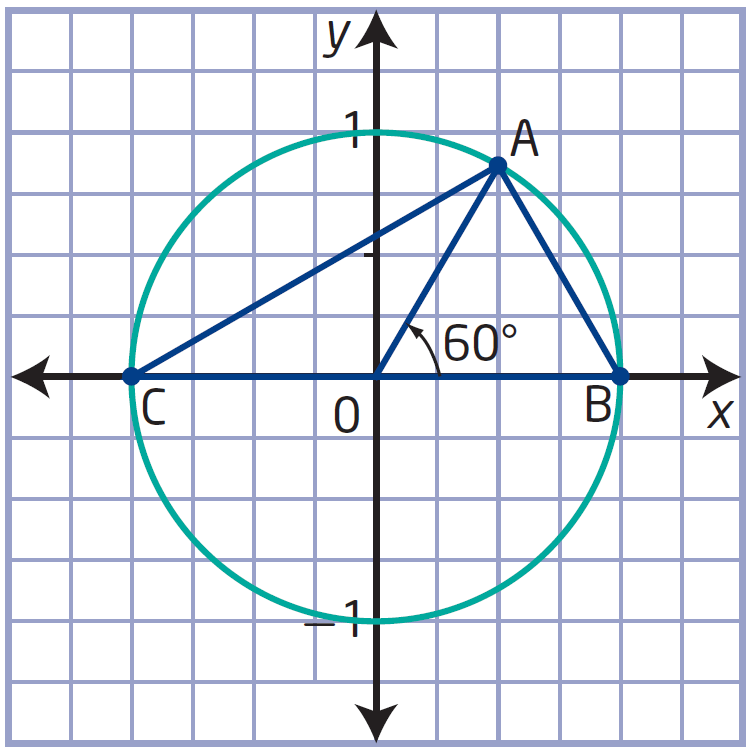
\includegraphics[width=2in]{figures/pyth-circle.png}
\]
}
\sol{
Since they are both radii, $OA=OB=1$.  Therefore, $\triangle OAB$ is isosceles with $\angle OAB=\angle ABO=60^{\circ}$. Hence $\triangle OAB$ is equilateral and $AB=1$, and $C B=2$.
\\[1em]
Since $OA$ is the terminal arm of $60^{\circ}$, the coordinates of $A$ are $\left(\frac{1}{2}, \frac{\sqrt{3}}{2}\right)$. The coordinates of $C$ are $(-1,0)$. Then, use the Pythagorean Theorem in the right triangle with hypotenuse $AC$.
\begin{align*}
	AC^2 & =\left(\frac{\sqrt{3}}{2}\right)^2+\left(\frac{3}{2}\right)^2 \\
	AC^2 & =\frac{3}{4}+\frac{9}{4}                                      \\
	AC^2 & =3                                                            \\
	AC   & =\sqrt{3}
\end{align*}
Then, in $\angle ABC$, $BC^2=4$, and
\[
	AC^2+AB^2 =3+1=4
\]
So the sides of $\triangle ABC$ satisfy the Pythagorean Theorem, with $\angle CAB=90^{\circ}$ because $\mathrm{BC}$ is the hypotenuse.
}
\chapter{The Sine Law and Cosine Law}
Solving a triangle without the Sine Law:
\\[10em]
Solving a triangle with the Sine Law:
\\[10em]
When you can use the Sine Law:
\\[10em]
\clearpage 
Proof of the Sine Law:
\\[300em]
The Ambiguous Case:
\\[5em]
The ambiguous case occurs when:
\clearpage 
The Cosine Law:
\\[10em]
When you can use the Cosine Law:
\\[10em]
Proof of the Cosine Law:
\vfill 
\[
\begin{array}{|c|l|}
\hline \text { Given } & \text { Method of Solving } \\
\hline \text { ASA or AAS } & \begin{array}{l}
\text { 1. Find the remaining angle using } \angle A+\angle B+\angle C=180^{\circ} . \\
\text { 2. Find the remaining sides using the Law of Sines. }
\end{array} \\
\hline \multirow{2}{*}{\text { ASS }} & \begin{array}{l}
\text { Be aware of the ambiguous case. There may be two solutions. } \\
\text { 1. Find an angle using the Law of Sines. } \\
\text { 2. Find the remaining angle using } \angle A+\angle B+\angle C=180^{\circ} . \\
\text { 3. Find the remaining side using the Law of Sines. }
\end{array} \\
\hline \text { SAS } & \begin{array}{l}
\text { 1. Find the remaining side using the Law of Cosines. } \\
\text { 2. Find the smaller of the two remaining angles using the Law of Sines. } \\
\text { 3. Find the remaining angle using } \angle A+\angle B+\angle C=180^{\circ} .
\end{array} \\
\hline \multirow{2}{*}{\text { SSS }} & \begin{array}{l}
\text { 1. Find the largest angle using the Law of Cosines. } \\
\text { 2. Find the remaining angle by using the Law of Sines. } \\
\text { 3. Find the remaining angle using } \angle A+\angle B+\angle C=180^{\circ} .
\end{array} \\
\hline
\end{array}
\]
	\clearpage 
\section*{Examples}
\clearpage \ 
\clearpage 
\prb{Is a triangle with sides measuring 10, 4, and 5 possible? Explain.}
\sol{No. The two shorter sides combined must be longer than the longest side.}
\prb{In $\triangle A B C, \angle A=65^{\circ}, \angle B=62^{\circ}$. What side of the triangle is the shortest? What side is the longest?}
\sol{Side $c$ is the shortest and $a$ is the longest side. The shortest side is opposite the smallest angle $\left(\angle C=53^{\circ}\right)$, and the longest side is opposite the largest angle $\left(\angle A=65^{\circ}\right)$.}
\prb{
	Explain why no triangle is possible with the given information.
	\begin{tasks}(2)
		\task
		\vspace{-2.2em}
		\[
			\begin{array}{lll}
				A=38^{\circ} & B=69^{\circ} & C=73^{\circ} \\
				a=12         & b=14         & c=13
			\end{array}
		\]
		\vspace{5em}
		\task
		\vspace{-2.2em}
		\[
			\begin{array}{lll}
				A=42^{\circ} & B=65^{\circ} & C=70^{\circ} \\
				a=7          & b=11         & c=12
			\end{array}
		\]
		\vspace{5em}
		\task
		\vspace{-2.2em}
		\[
			\begin{array}{lll}
				A=39^{\circ} & B=46^{\circ} & C=95^{\circ} \\
				a=5          & b=6          & c=12         \\
			\end{array}
		\]
		\vspace{5em}
		\task
		\vspace{-2.2em}
		\[
			\begin{array}{lll}
				A=120^{\circ} & B=20^{\circ} & C=40^{\circ} \\
				a=12          & b=6          & c=12
			\end{array}
		\]
		\vspace{5em}
	\end{tasks}
}
\sol{
	\begin{tasks}(2)
		\task The largest angle $\left(\angle C=73^{\circ}\right)$ must have the largest side opposite it. This is not the case.
		\task The three angles do not add up to $180^{\circ}$.
		\task The two smaller sides added are less than the largest side.
		\task Two angles of different degrees, $\angle A$ and $\angle C$, cannot have sides of the same value.
	\end{tasks}
}
\prb{
	Find the angle that has the same sine ratio as following, with the restriction of $0^{\circ} \leq \theta \leq 180^{\circ}$.
	\begin{tasks}(2)
		\task $\sin 10^{\circ}$
		\vspace{2em}
		\task $\sin 30^{\circ}$
		\vspace{2em}
		\task $\sin 42^{\circ}$
		\vspace{2em}
		\task $\sin 71^{\circ}$
		\vspace{2em}
		\task $\sin 121^{\circ}$
		\vspace{2em}
		\task $\sin 137^{\circ}$
		\vspace{2em}
	\end{tasks}
}
\sol{
	\begin{tasks}(6)
		\task $170^{\circ}$
		\task $150^{\circ}$
		\task $138^{\circ}$
		\task $109^{\circ}$
		\task $59^{\circ}$
		\task $43^{\circ}$
	\end{tasks}
}
\prb{
	Determining the lengths of all three sides and the measures of all three angles is called solving a triangle. Solve each triangle.
	\begin{tasks}(2)
		\task \\
		\incfig[0.8]{triangle1}
		\vspace{8em}
		\task \\
		\incfig[0.8]{triangle2}
		\vspace{8em}
		\task \\
		\incfig[0.8]{triangle3}
		\vspace{8em}
		\task \\
		\incfig[0.8]{triangle4}
		\vspace{8em}
	\end{tasks}
}
\sol{
	\begin{tasks}(1)
		\task
		This is an ambiguous case.
		First find the acute measure of $\angle \mathrm{C}$ :
		\begin{align*}
			\frac{\sin \mathrm{C}}{c}  & =\frac{\sin \mathrm{B}}{b}                            \\
			\frac{\sin \mathrm{C}}{13} & =\frac{\sin 67^{\circ}}{12}                           \\
			\sin \mathrm{C}            & =\frac{13 \sin 67^{\circ}}{12}                        \\
			\angle \mathrm{C}          & =\sin ^{-1}\left(\frac{13 \sin 67^{\circ}}{12}\right) \\
			\angle \mathrm{C}          & =85.721 \ldots
		\end{align*}
		The acute measure of $\angle \mathrm{C}$ is $86^{\circ}$, to the nearest degree. Then, the obtuse measure of $\angle \mathrm{C}$ is $180^{\circ}-85.721^{\circ}=94.279 \ldots \circ$. The obtuse measure of $\angle \mathrm{C}$ is $94^{\circ}$, to the nearest degree.
		\\
		Then, find the measure of $\angle \mathrm{A}$.
		\[
			\begin{array}{lll}
				\angle \mathrm{A}=180^{\circ}-\left(85.721 \ldots{ }^{\circ}+67^{\circ}\right) & \text { or }                               & \angle \mathrm{A}=180^{\circ}-\left(94.279 \ldots{ }^{\circ}+67^{\circ}\right) \\
				\angle \mathrm{A}=27.279 \ldots{ }^{\circ}                                     & \angle \mathrm{A}=18.721 \ldots{ }^{\circ}
			\end{array}
		\]
		The measure of $\angle \mathrm{A}$ is $27^{\circ}$ or $19^{\circ}$, to the nearest degree.
		Now find the measure of side $a$.
		\[
			\begin{array}{rlrl}
				\frac{a}{\sin \mathrm{A}}              & =\frac{b}{\sin \mathrm{B}} \quad \text { or }             & \frac{a}{\sin \mathrm{A}}               & =\frac{b}{\sin \mathrm{B}}                                \\
				\frac{a}{\sin 27.279 \ldots 0^{\circ}} & =\frac{12}{\sin 67^{\circ}}                                                                                                                                     \\
				a                                      & =\frac{12 \sin 27.279 \ldots{ }^{\circ}}{\sin 67^{\circ}} & \frac{a}{\sin 18.721 \ldots{ }^{\circ}} & =\frac{12}{\sin 67^{\circ}}                               \\
				a                                      & =5.974 \ldots                                             & a                                       & =\frac{12 \sin 18.721 \ldots{ }^{\circ}}{\sin 67^{\circ}} \\
				a                                      & =4.184 \ldots
			\end{array}
		\]
		Summary:\\
		Acute case: $\angle \mathrm{C}=86^{\circ}, \angle \mathrm{A}=27^{\circ}$, side $a$ is $6.0 \mathrm{~m}$, to the nearest tenth of a metre.
		Obtuse case: $\angle \mathrm{C}=94^{\circ}, \angle \mathrm{A}=19^{\circ}$, side $a$ is $4.2 \mathrm{~m}$, to the nearest tenth of a metre.
		$<$ Note: If you use the rounded degree values, then $a$ is $5.9 \mathrm{~m}$ for the acute case. For the obtuse case, using rounded degree values results in the same answer.
		\task
		$\angle \mathrm{C}=54^{\circ}$.
		The length of side $a$ is $33.6 \mathrm{~m}$, to the nearest tenth of a metre.
		The length of side $c$ is $40.7 \mathrm{~m}$, to the nearest tenth of a metre.
		\task
		$\angle \mathrm{B}=119^{\circ}$.
		The length of side $a$ is $12.4 \mathrm{~mm}$, to the nearest tenth of a millimetre.
		The length of side $c$ is $20.9 \mathrm{~mm}$, to the nearest millimetre.
		\task
		$\angle B=71^{\circ}$.
		The length of side $a$ is $16.5 \mathrm{~cm}$, to the nearest tenth of a centimetre.
		The length of side $c$ is $19.4 \mathrm{~cm}$, to the nearest centimetre.
	\end{tasks}
}
\prb{The Canadian Coast Guard Pacific Region is responsible for more than 27 000 km of coastline. The rotating spotlight from the Coast Guard ship can illuminate up to a distance of 250 m. An observer on the shore is 500 m from the ship. His line of sight to the ship makes an angle of 20° with the shoreline. What length of shoreline is illuminated by the spotlight?
	\includegraphics*[width=3in]{coastguard}
}
\sol{
	Let $\mathrm{C}$ be the position of the coast guard ship and $\mathrm{H}$ the foot of the perpendicular from $\mathrm{C}$ to the shoreline.
	\begin{align*}
		\frac{\sin \mathrm{D}}{500} & =\frac{\sin 20^{\circ}}{250}                            \\
		\sin \mathrm{D}             & =\frac{500 \sin 20^{\circ}}{250}                        \\
		\angle \mathrm{D}           & =\sin ^{-1}\left(\frac{500 \sin 20^{\circ}}{250}\right) \\
		\angle \mathrm{D}           & =43.160 \ldots
	\end{align*}
	Then, in $\triangle \mathrm{CDH}$ :
	\begin{align*}
		\cos 43.160 \ldots{ }^{\circ} & =\frac{\mathrm{DH}}{250}           \\
		\mathrm{DH}                   & =250 \cos 43.160 \ldots{ }^{\circ} \\
		\mathrm{DH}                   & =182.361 \ldots
	\end{align*}
	Since $\mathrm{CA}=\mathrm{CD}, \Delta \mathrm{ACH} \approx \triangle \mathrm{DCH}$ and $\mathrm{AH}+\mathrm{HD}$.
	So $\mathrm{AD}=2(182.361 \ldots)$ or $364.722 \ldots$
	The length of shoreline that is illuminated by the spotlight is $364.7 \mathrm{~m}$, to the nearest tenth of a metre.
}
\clearpage
\prb{
	Determine whether the Law of Sines or the Law of Cosines would be used to begin the solution process for each triangle.
	\begin{tasks}(2)
		\task \\ \incfig[0.8]{cosine-law-1} \vspace{8em}
		\task \\ \incfig[0.8]{cosine-law-2} \vspace{8em}
		\task \\ \incfig[0.8]{cosine-law-3} \vspace{8em}
		\task \\ \incfig[0.8]{cosine-law-4} \vspace{8em}
		\task \\ \incfig[0.8]{cosine-law-5} \vspace{8em}
		\task \\ \incfig[0.8]{cosine-law-6} \vspace{8em}
	\end{tasks}
}
\sol{
	\begin{tasks}(3)
		\task Law of Cosines
		\task Law of Sines
		\task none
		\task Law of Sines
		\task Law of Cosines 
		\task Law of Sines
	\end{tasks}
}
\prb{
	Solve the triangle using the Law of Cosines. Round answers to one decimal place.  A drawing is very helpful.
	\begin{tasks}(2) 
		\task $\angle A=50^{\circ}, b=10, c=15$
		\vspace{12em}
		\task $\angle B=36^{\circ}, a=4, c=10$
		\vspace{12em}
		\task $\angle C=60^{\circ}, b=4, a=8$
		\vspace{12em}
		\task $a=2, b=3, c=4$
		\vspace{12em}
		\task $a=7, b=24, c=25$
		\vspace{12em}
		\task $a=9, b=14, c=11$
		\vspace{12em}
		\task $y=4, z=1, \angle X=120^{\circ}$
		\vspace{12em}
		\task $x=6, y=7, z=13$
		\vspace{12em}
		\task $\angle S=127.8^{\circ}, k=1578, d=2654$
		\vspace{12em}
		\task $s=1504, q=2365, r=1953$
		\vspace{12em}
	\end{tasks}
}
\sol{
	\begin{tasks}(2)
		\task $\angle B=41.8^{\circ}, \angle C=88.2^{\circ}, a=11.5$
		\task $\angle A=19.2^{\circ}, \angle C=124.8^{\circ}, a=7.2$
		\task $\angle A=90^{\circ}, \angle B=30^{\circ}, c=6.9$
		\task $\angle A=29.0^{\circ}, \angle B=46.5^{\circ}, \angle C=104.5^{\circ}$
		\task $\angle A=16.3^{\circ}, \angle B=73.7^{\circ}, \angle C=90^{\circ}$
		\task $\angle A=40^{\circ}, \angle B=88.3^{\circ}, \angle C=51.7^{\circ}$
		\task $\angle Y=49.1^{\circ}, \angle Z=10.9^{\circ}, x=4.6$
		\task Impossible triangle.
		\task $\angle D=33.2^{\circ}, \angle K=19.0^{\circ}, s=3829.8$
		\task $\angle Q=85.3^{\circ}, \angle R=55.4^{\circ}, \angle S=39.3^{\circ}$
	\end{tasks}
}
\begin{Exercise}
	Solve each triangle using the Law of Sines. If two triangles exist, solve both completely. A drawing is very helpful.
	% \vspace{-3em}
	\begin{tasks}(2)
		\task $\angle A=140^{\circ}, \angle C=25^{\circ}, a=20$
		\vspace{14em}
		\task $\angle B=38^{\circ}, b=8, a=6$
		\vspace{14em}
		\task $\angle C=27^{\circ}, \angle B=46^{\circ}, a=120$
		\vspace{14em}
		\task $\angle A=110^{\circ}, a=24, b=25$
		\vspace{14em}
		\task $\angle B=60^{\circ}, b=4 \sqrt{3}, a=8$
		\vspace{14em}
		\task $\angle C=41^{\circ}, c=9, a=9$
		\vspace{14em}
		\task $\angle A=74^{\circ}, a=7, b=8.1$
		\vspace{14em}
		\task $\angle A=58^{\circ}, \angle B=48^{\circ}, b=30.5$
		\vspace{14em}
		\task $\angle A=43^{\circ}, \angle B=38^{\circ}, c=17.2$
		\vspace{14em}
		\task $\angle A=33^{\circ}, a=27.2, b=12.4$
		\vspace{14em}
		\task $\angle A=30^{\circ}, a=8, b=10$
		\vspace{14em}
		\task $\angle A=58^{\circ}, a=9, b=10$
		\vspace{14em}
		\task $\angle A=10^{\circ}, \angle B=60^{\circ}, a=4.5$
		\vspace{14em}
		\task $\angle B=10^{\circ}, \angle C=135^{\circ}, c=60$
		\vspace{14em}
		\task $\angle C=52^{\circ}, c=8.5, b=12.4$
		\vspace{14em}
		\task $\angle B=27, b=2, c=5$
		\vspace{14em}
	\end{tasks}
\end{Exercise}
\sol{
	\begin{tasks}(2)
		\task $\angle B=15^{\circ}, b=8.1, c=13.1$
		\task $\angle A=27.5^{\circ}, \angle C=114.5^{\circ}, c=11.8$
		\task $\angle A=107^{\circ}, b=90.3, c=57.0$
		\task Impossible triangle.
		\task $\angle A=90^{\circ}, \angle C=30^{\circ}, c=4$
		\task $\angle A=41^{\circ}, \angle B=98^{\circ}, b=13.6$
		\task Impossible triangle.
		\task $\angle C=74^{\circ}, a=34.8, c=39.5$
		\task $\angle C=99^{\circ}, a=11.9, b=10.7$ 
		\task $\angle B=14.4^{\circ}, \angle C=132.6^{\circ}, c=36.7$
		\task* $\angle B=38.7^{\circ}, 141.3^{\circ}, \angle C=111.3^{\circ}, 8.7^{\circ}, c=14.9 .2 .4$
		\task* $\angle B=70.4^{\circ}, 109.6^{\circ}, \angle C=51.6^{\circ}, 12.4^{\circ}, c=8.3,2.3$
		\task $\angle C=110^{\circ}, b=22.4, c=24.4$
		\task $\angle A=35^{\circ}, a=48.7, b=14.7$
		\task Impossible triangle.
		\task Impossible triangle.
	\end{tasks}
}
\prb{
	Solve $\triangle A B C$ using either the Law of Sines or the Law of Cosines to begin the solution.
\begin{tasks}(2)
	\task $\angle A=126^{\circ}, b=9, c=12.2$
	\vspace{10em}
	\task $\angle A=28^{\circ}, \angle B=42^{\circ}, c=18.2$
	\vspace{10em}
	\task $\angle B=63^{\circ}, b=8, c=10$
	\vspace{10em}
	\task $\angle B=41^{\circ}, a=11, c=6$
	\vspace{10em}
	\task $a=12.3, b=9.6, c=8.9$
	\vspace{10em}
	\task $\angle C=38^{\circ}, b=9, c=7$
	\vspace{10em}
	\task $\angle C=100^{\circ}, a=10, c=10$
	\vspace{10em}
	\task $\angle A=60^{\circ}, a=2 \sqrt{3}, c=4$
	\vspace{10em}
	\task $a=1.32, b=0.88, c=0.65$
	\vspace{10em}
	\task $\angle A=75^{\circ}, b=4-2 \sqrt{3}, a=\sqrt{6}-\sqrt{2}$
	\vspace{10em}
\end{tasks}
}
\sol{
	\begin{tasks}(2)
		\task $\angle B=22.6^{\circ}, \angle C=31.4^{\circ}, a=18.9$
		\task $\angle C=110^{\circ}, a=9.1, b=13.0$
		\task Impossible triangle.
		\task $\angle A=107.7^{\circ}, \angle C=31.3^{\circ}, b=7.6$
		\task $\angle A=83.3^{\circ}, \angle B=50.8^{\circ}, \angle C=45.9^{\circ}$
		\task $\angle A=89.7^{\circ}, 14.3^{\circ}, \angle B=52.3^{\circ}, 127.7^{\circ}, a=11.4,2.8$
		\task Impossible triangle.
		\task $\angle B=30^{\circ}, \angle C=90^{\circ}, b=2$
		\task $\angle A=118.5^{\circ}, \angle B=35.9^{\circ}, \angle C=25.6^{\circ}$
		\task $\angle B=30^{\circ}, \angle C=75^{\circ}, c=\sqrt{6}-\sqrt{2}$
	\end{tasks}
}
\clearpage
\prb{A plane is sighted by two observers $1 \mathrm{~km}$ apart at angles $74^{\circ}$ and $78^{\circ}$. How high is the plane?}
\vfill
\sol{13.48 km}
\prb{A hot air balloon is flying directly between two cities that are $4 \mathrm{~km}$ apart. The balloonist finds that the angle of depression to one city is $38^{\circ}$ and $33^{\circ}$ to the other city. How high above the ground is the balloon?}
\vfill
\sol{1.42 km}
\prb{
Two planes leave airport $A$ in different directions. One plane lands at airport $B, 630 \mathrm{~km}$ from airport $A$. The other plane lands at airport $\mathrm{C}$ some time later. If $\angle A B C=110^{\circ}$ and $\angle A C B=40^{\circ}$, how far did the second plane fly?
}
\vfill
\clearpage
\sol{
	921 km
}
\prb{
	A plane flies $420 \mathrm{~km}$ from point $A$ at a direction of $135^{\circ}$ from due east and then travels $240 \mathrm{~km}$ at a direction of $240^{\circ}$ from due east. How far is the plane from point $A$ ?
	\vspace{10em}
}
\sol{
	$426.4 \mathrm{~km}$
}
\prb{
In a solar system, the distance from the Sun $(S)$ to planets $A$ and $B$ are 85 and 61 million miles respectively. When $\angle A=20^{\circ}$, how far is it from planet $A$ to planet $B$ and $B^{\prime}$?\\[1em]
\incfig[0.25]{solar}
}
\vfill
\sol{
	$A B^{\prime}=133.6$ million miles
	$A B=26.4$ million miles
}
\prb{
Three circles with radius $A=4 \mathrm{~cm}, B=3 \mathrm{~cm}$, and $C=5 \mathrm{~cm}$ are shown. If $\angle C A B=35^{\circ}$, how far is it from the centre of circle $A$ to the centre of circle $C$?\\[1em]
\incfig[0.35]{circles}
}
\vfill
\clearpage
\sol{
	$12.65 \mathrm{~cm}$
}
\prb{
	Three circles of radius 3,5 , and $7 \mathrm{~cm}$ are tangent to each other. Find the largest angle formed by joining their centres.
\vspace{10em}
	}
\sol{
	$82.8^\circ$
}
\prb{
	The rectangular box has dimensions $4 \mathrm{~cm} \times 3 \mathrm{~cm} \times 2 \mathrm{~cm}$. Find angle $\theta$ formed by a diagonal of the base, and a diagonal of the $2 \mathrm{~cm} \times 3 \mathrm{~cm}$ side.
	\\ \[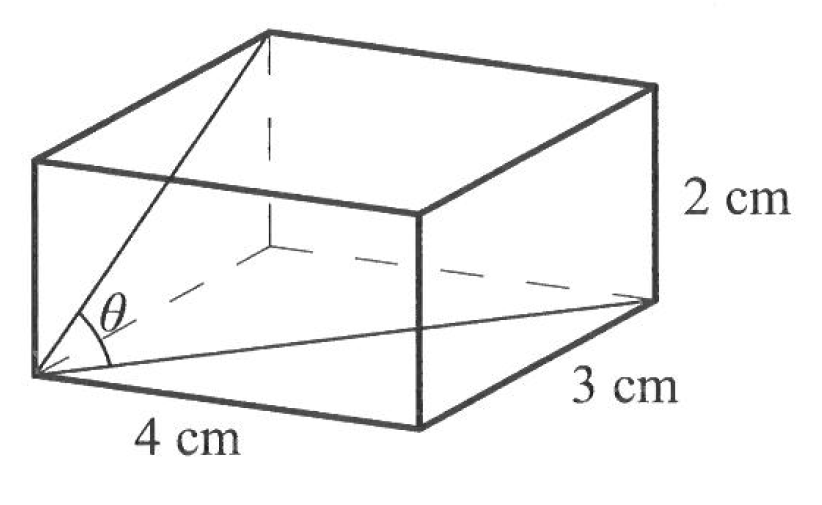
\includegraphics[width=2in]{figures/diagonal-box.png}\]
}
\chapter{Volume and Surface Area}
Volume of a prism:
\vfill 
Volume of a pyramid:
\vfill 
Volume of a cylinder:
\vfill 
Volume of a cone:
\vfill 
Surface area of a cone:
\vfill
\clearpage 
\section*{Examples}
\clearpage \ 
\clearpage
\begin{Exercise} %Mickelson 10: 1.4 #1
	Find the surface area and volume of each prism.
	\begin{tasks}(2)
		\task \vspace{-2.5em}\[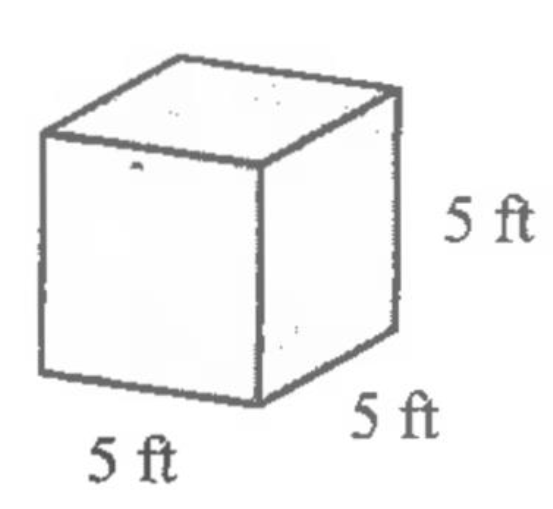
\includegraphics[width=0.5\columnwidth]{figures/cube1.png}\]
		\vspace{2.5em}
		\task \vspace{-2.5em}\[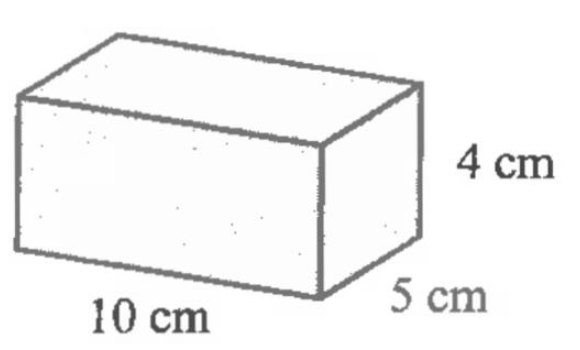
\includegraphics[width=0.5\columnwidth]{figures/prism2.png}\]
		\vspace{2.5em}
		\task \vspace{-2.5em}\[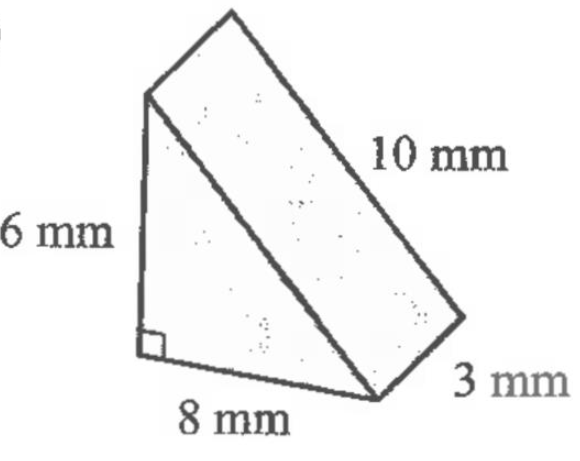
\includegraphics[width=0.5\columnwidth]{figures/prism3.png}\]
		\vspace{2.5em}
		\task \vspace{-2.5em}\[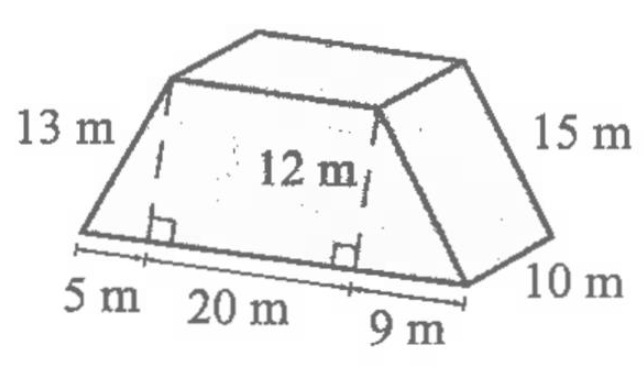
\includegraphics[width=0.5\columnwidth]{figures/prism4.png}\]
		\vspace{2.5em}
		\task \vspace{-2.5em}\[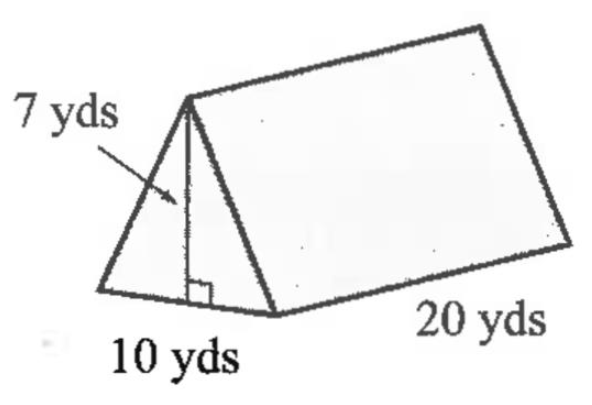
\includegraphics[width=0.5\columnwidth]{figures/prism5.png}\]
		\vspace{2.5em}
		\task \vspace{-2.5em}\[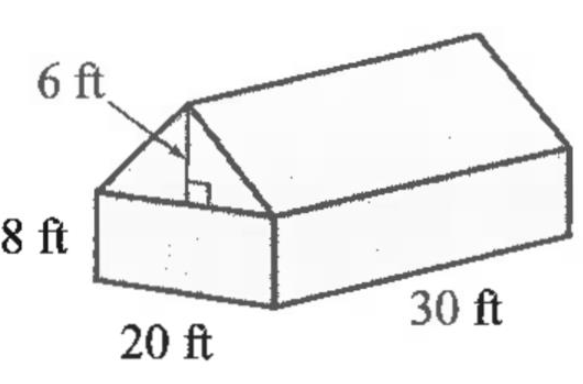
\includegraphics[width=0.5\columnwidth]{figures/prism6.png}\]
		\vspace{2.5em}
		\task \vspace{-2.5em}\[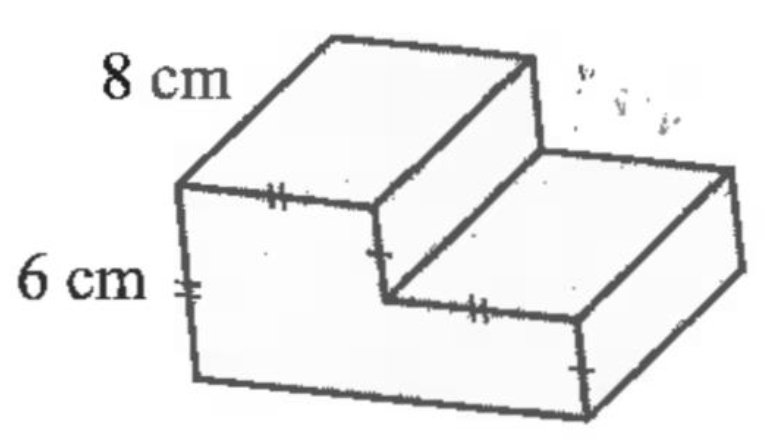
\includegraphics[width=0.5\columnwidth]{figures/prism7.png}\]
		\vspace{2.5em}
		\task \vspace{-2.5em}\[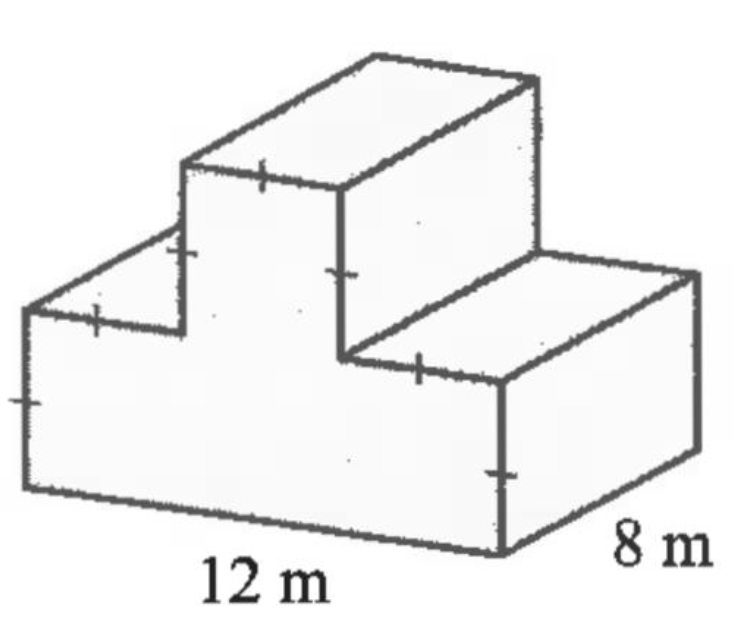
\includegraphics[width=0.5\columnwidth]{figures/prism8.png}\]
		\vspace{2.5em}
		\task \vspace{-2.5em}\[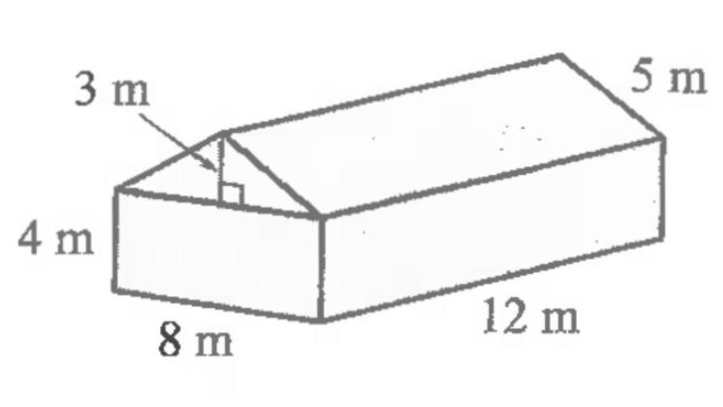
\includegraphics[width=0.5\columnwidth]{figures/prism9.png}\]
		\vspace{2.5em}
		\task \vspace{-2.5em}\[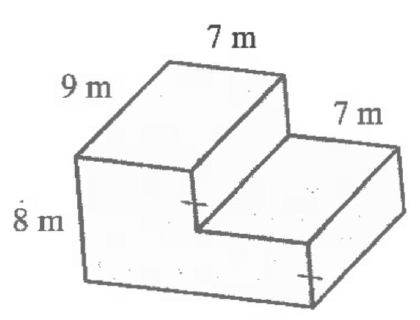
\includegraphics[width=0.5\columnwidth]{figures/prism11.png}\]
		\vspace{2.5em}
		\task \vspace{-2.5em}\[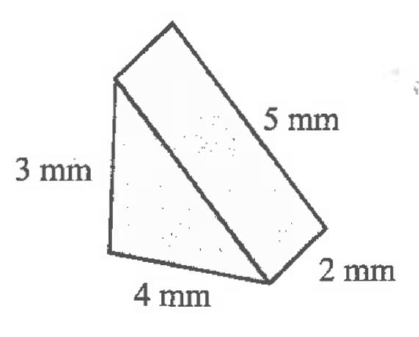
\includegraphics[width=0.5\columnwidth]{figures/prism12.png}\]
		\vspace{2.5em}
		\task \vspace{-2.5em}\[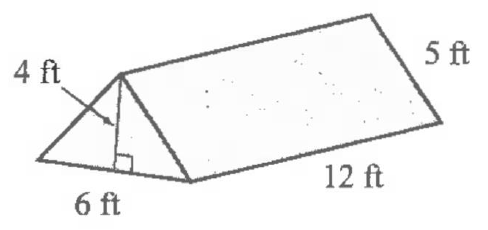
\includegraphics[width=0.5\columnwidth]{figures/prism13.png}\]
		\vspace{2.5em}
	\end{tasks}
\end{Exercise}
\sol{
	\begin{tasks}(2)
	\task $150 \mathrm{ft}^2, 125 \mathrm{ft}^3$
	\task $220 \mathrm{~cm}^2, 200 \mathrm{~cm}^3$
	\task $120 \mathrm{~mm}^2, 72 \mathrm{~mm}^3$
	\task $1468 \mathrm{~m}^2, 3240 \mathrm{~m}^3$
	\task $614.1 \mathrm{yd}^2, 700 \mathrm{yd}^3$
	\task $2219.7 \mathrm{ft}^2, 6600 \mathrm{ft}^3$
	\task $396 \mathrm{~cm}^2, 432 \mathrm{~cm}^3$
	\task $448 \mathrm{~m}^2, 512 \mathrm{~m}^3$
	\task $400 \mathrm{~m}^2, 528 \mathrm{~m}^3$
	\task $564 \mathrm{~m}^2, 756 \mathrm{~m}^3$
	\task $36 \mathrm{~mm}^2, 12 \mathrm{~mm}^3$
	\task $216 \mathrm{ft}^2, 144 \mathrm{ft}^3$
	\end{tasks}
}
\prb{ %2
	An Olympic size swimming pool is $50 \mathrm{~m}$ long, $21 \mathrm{~m}$ wide and $2 \mathrm{~m}$ deep. How many litres of water are needed to fill the pool? $\left(1 \mathrm{~m}^3=1000 l\right)$
}
\sol{
	2100000 L
}
\vspace{4em}
\prb{%18
	A regular hexagonal based prism has sides of $4 \mathrm{~cm}$ and a height of $5 \mathrm{~cm}$.
	\begin{tasks}(2)
		\task What is the surface area of the prism?
		\task What is the volume of the prism?
	\end{tasks}
}
\sol{
	\begin{tasks}(2)
	\task $48 \sqrt{3}+120 \approx 203.14 \mathrm{~cm}^2$
	\task $120 \sqrt{3} \approx 207.84 \mathrm{~m}^3$
	\end{tasks}
}
\clearpage
\prb{%21
	Find the volume of a right triangular prism with height $2(x+1)$. The base is an isosceles right triangle with a hypotenuse of $\sqrt{2} x$.
}
\sol{
	$x^3+x^2$
}
\vspace{5em}
\prb{ %Mickelson 10: 1.5 #3
	\begin{tasks}(2) Find the volume of each pyramid.
		\task \vspace{-2.5em}\[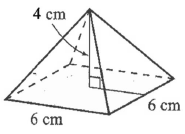
\includegraphics[width=0.5\columnwidth]{figures/pyramid1.png}\]\vspace{5em}
		\task \vspace{-2.5em}\[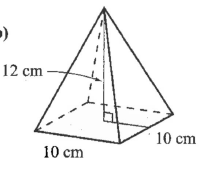
\includegraphics[width=0.5\columnwidth]{figures/pyramid2.png}\]\vspace{5em}
		\task \vspace{-2.5em}\[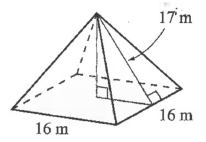
\includegraphics[width=0.5\columnwidth]{figures/pyramid3.png}\]\vspace{5em}
		\task \vspace{-2.5em}\[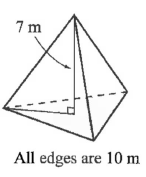
\includegraphics[width=0.5\columnwidth]{figures/pyramid4.png}\]\vspace{5em}
	\end{tasks}
}
\sol{
	\begin{tasks}(2)
		\task $96 \mathrm{~cm}^2, 48 \mathrm{~cm}^3$
		\task $360 \mathrm{~cm}^2, 400 \mathrm{~cm}^3$
		\task $800 \mathrm{~m}^2, 1280 \mathrm{~m}^3$
		\task $173.2 \mathrm{~m}^2, 101.0 \mathrm{~m}^3$
	\end{tasks}
}
\prb{%4
	What is the ratio of the volume of the pyramid to the volume of the rectangular solid?\\[2em]
	\vspace{-2.5em}\[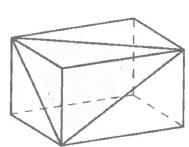
\includegraphics[width=0.3\columnwidth]{figures/pyramidratio.png}\]
}
\sol{
	$1:6$
}
\clearpage
\prb{%7
	A regular hexagonal pyramid has base edges of length $1 \mathrm{~cm}$, and lateral edges of length $2 \mathrm{~cm}$.
	\begin{tasks}(2)
		\task What is the volume of the pyramid?
		\task What is the surface area of the pyramid?
	\end{tasks}}
\sol{
	\begin{tasks}(2)
		\task $V=\frac{1}{3}\left(A_{\text {base }}\right)(h)=\frac{1}{3}\left(\frac{3 \sqrt{3}}{2}\right)(\sqrt{3})=\frac{3}{2} \mathrm{~cm}^2$
		\task $S . A .=$ area of base $+6$ sides $=\frac{3 \sqrt{3}}{2}+6\left(\frac{1}{2} \cdot 1 \cdot \frac{\sqrt{15}}{2}\right)=\left(\frac{3 \sqrt{3}}{2}+\frac{3 \sqrt{15}}{2}\right) \approx 8.41 \mathrm{~cm}^2$
	\end{tasks}
}
\vspace{5em}
\prb{%14
	If you double all the dimensions of a pyramid, what does it do to the surface area? Volume?
}
\sol{Surface Area is 4 times as large. Volume is 8 times as large.}
\vspace{5em}
\prb{%17
	A pyramid has a rectangular base with length twice the width. If the height is $6 \mathrm{~cm}$ and the volume is $256 \mathrm{~cm}^3$, what are the dimensions of the rectangular base?
}
\sol{
	$V=\frac{1}{3}\left(A_{\text {base }}\right)(h) \rightarrow 256=\frac{1}{3}(x \cdot 2 x)(6) \rightarrow x^2=64 \rightarrow x=8 ;$ Therefore $8 \mathrm{~cm} \times 16 \mathrm{~cm}$
}
\begin{Exercise}
	% Mickelson 1.6 #1
	Calculate the surface area and volume of each figure.
	\begin{tasks}(2)
		\task \vspace{-2.5em}\[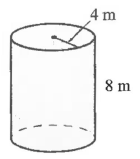
\includegraphics[scale=0.8]{figures/volume1.png}\]
		\vspace{5em}
		\task \vspace{-2.5em}\[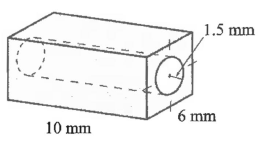
\includegraphics[scale=0.8]{figures/volume2.png}\]
		\vspace{5em}
		\task \vspace{-2.5em}\[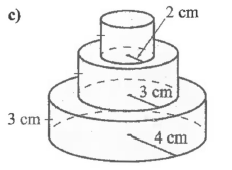
\includegraphics[scale=0.8]{figures/volume3.png}\]
		\vspace{5em}
		\task \vspace{-2.5em}\[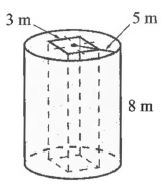
\includegraphics[scale=0.8]{figures/volume4.png}\]
		\vspace{5em}
		\task \vspace{-2.5em}\[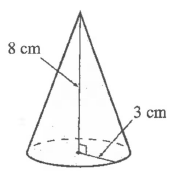
\includegraphics[scale=0.8]{figures/volume5.png}\]
		\vspace{5em}
		\task \vspace{-2.5em}\[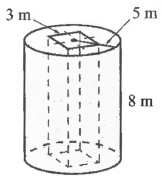
\includegraphics[scale=0.8]{figures/volume6.png}\]
		\vspace{5em}
		\task \vspace{-2.5em}\[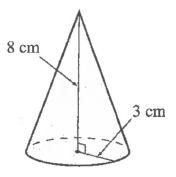
\includegraphics[scale=0.8]{figures/volume7.png}\]
		\vspace{5em}
		\task \vspace{-2.5em}\[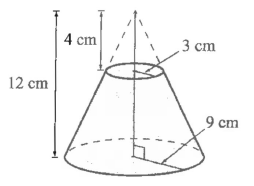
\includegraphics[scale=0.8]{figures/volume8.png}\]
		\vspace{5em}
		\task \vspace{-2.5em}\[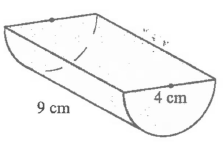
\includegraphics[scale=0.8]{figures/volume9.png}\]
		\vspace{5em}
		\task \vspace{-2.5em}\[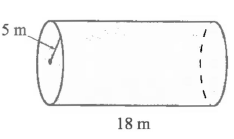
\includegraphics[scale=0.8]{figures/volume10.png}\]
		\vspace{5em}
		\task \vspace{-2.5em}\[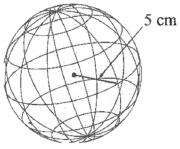
\includegraphics[scale=0.8]{figures/volume11.png}\]
		\vspace{5em}
		\task \vspace{-2.5em}\[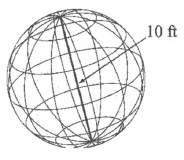
\includegraphics[scale=0.8]{figures/volume12.png}\]
		\vspace{5em}
	\end{tasks}
\end{Exercise}
\sol{
	\begin{tasks}(2)
		\task $301.6 \mathrm{~m}^2, 402.1 \mathrm{~m}^3$
		\task $392.1 \mathrm{~mm}^2, 289.3 \mathrm{~mm}^3$
		\task $270.2 \mathrm{~m}^2, 273.3 \mathrm{~m}^3$
		\task $486.4 \mathrm{~m}^2, 556.3 \mathrm{~m}^3$
		\task $108.8 \mathrm{~cm}^2, 75.4 \mathrm{~cm}^3$
		\task $659.73 \mathrm{~cm}^2, 980.18 \mathrm{~cm}^3$
		\task $105.11 \mathrm{~cm}^2, 56.55 \mathrm{~cm}^3$
		\task $722.57 \mathrm{~m}^2, 1413.72 \mathrm{~m}^3$
		\task $314.16 \mathrm{~cm}^2, 523.60 \mathrm{~cm}^3$
		\task $314.16 \mathrm{ft}^2, 523.60 \mathrm{ft}^3$
	\end{tasks}
}
\prb{
	%3
	Soup is sold in two can sizes. The can is cylindrical in shape. The height of can $A$ is twice the height of can $B$. The radius of can $B$ is twice the radius of can $A$. Can $B$ costs twice as much as can $A$. Which can is the better buy?
}
\sol{
	Can B holds twice the volume of can A, so they are of equal value.
}
\vspace{8em}
\prb{
	%5
	If rectangle $\mathrm{ABCD}$ is is revolved about the line $\mathrm{AD}$, what is the volume of the space through which it moves?\\[1em]
	\[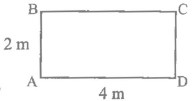
\includegraphics[scale=0.8]{figures/revolving-rectangle.png}\]
}
\vspace{5em}
\prb{%17
	A cylindrical block of cheese has a $60^{\circ}$ slice removed. If the volume of the removed slice is $18 \pi \mathrm{cm}^3$, what is the height of the block of cheese?
}
\sol{
	$V=\frac{1}{6} \pi r^2 h \rightarrow 18 \pi=\frac{1}{6} \pi \cdot 6^2 \cdot h \rightarrow h=3 \mathrm{~cm}$
}
\vspace{8em}
\prb{
	%24
	A hemispherical room requires four cans of paint to paint the floor. How many cans of paint are required to paint the walls?
}
\sol{
	$A=\pi r^2=4 \rightarrow r^2=\frac{4}{\pi} ; S . A .=2 \pi r^2=2 \pi \cdot \frac{4}{\pi}=8$ cans
}
\vspace{8em}
\prb{
	%25
	If a sphere and a cone have the same radius and volume, what must be the height of the cone in terms of the radius?
}
\sol{
	$\frac{4}{3} \pi r^3=\frac{1}{3} \pi r^2 h \quad \rightarrow \quad h=4 r$
}
\clearpage
\prb{
	%27
	A sphere with a radius of $4 \mathrm{~cm}$ has a $45^{\circ}$ section removed. What is the remaining surface area of the sphere?
}
\sol{
	S.A. $=\frac{7}{8}\left(4 \pi r^2\right)+\pi r^2=\frac{7}{8}\left(4 \pi \cdot 4^2\right)+\pi \cdot 4^2=72 \pi \approx 226.19 \mathrm{~cm}^2$
}
\vspace{8em}
\prb{
	%28
	A sphere fits exactly into a cube. What is the ratio of the surface area of the sphere to the surface area of the cube?
	\\ \[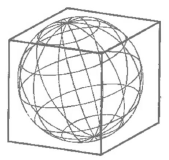
\includegraphics[scale=0.8]{figures/cubesphere.png}\]
}
\sol{
	$4 \pi r^2: 6(2 r)^2 \rightarrow 4 \pi r^2=24 r^2 \rightarrow \pi: 6$
}
\vspace{5em}
\prb{
	%29
	A sphere of radius $r$ is inscribed in a cone with diameter $A C=A B=B C$. Find the ratio of the volume of the sphere to the volume of the cone.
	\\ \[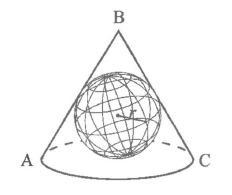
\includegraphics[scale=0.8]{figures/conesphere.png}\]
}
\sol{
	$\frac{4}{3} \pi r^3: \frac{1}{3} \pi R^2 h \rightarrow 4 r^3:(\sqrt{3} r)^2(3 r) \rightarrow 4 r^3: 9 r^3 \rightarrow 4: 9$
}
\vspace{5em}
\prb{
	%30
	Three tennis balls are packed tightly in different containers. What is the ratio of the volume of the tennis balls to the volume of the box in figures a, b and c?
	\begin{tasks}(3)
		\task \vspace{-2.5em}\[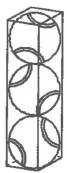
\includegraphics[scale=0.8]{figures/spherepack1.png}\]
		\task \vspace{-2.5em}\[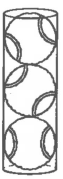
\includegraphics[scale=0.8]{figures/spherepack2.png}\]
		\task \vspace{-2.5em}\[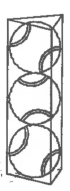
\includegraphics[scale=0.8]{figures/spherepack3.png}\]
	\end{tasks}
}
\sol{
	\begin{tasks}(1)
		\task $3\left(\frac{4}{3} \pi r^3\right):(2 r)(2 r)(6 r) \rightarrow 4 \pi r^3: 24 r^3 \rightarrow \pi: 6$
		\task $3\left(\frac{4}{3} \pi r^3\right): \pi \cdot r^2 \cdot 6 r \rightarrow 4 \pi r^3: 6 \pi r^3 \rightarrow 2: 3$
		\task $3\left(\frac{4}{3} \pi r^3\right): \frac{1}{2}(2 \sqrt{3} r)(3 r)(6 r) \rightarrow 4 \pi r^3: 18 \sqrt{3} r^3 \rightarrow 2 \pi: 9 \sqrt{3}$
	\end{tasks}
}
\clearpage \ 
\clearpage
\chapter{Selected Solutions.}
\shipoutAnswer
\end{document}
